% -*- mode: latex -*- %

\section{Experiments}
\label{sec:experiments}

We evaluate the benefits of the proposed methodology in simulation and on
real data. First, we study the effect of power tuning by comparing
power-tuned PPI (\ppipp) to both classical and prediction-powered inference
(PPI). We also compare to the original PPI approach for generic M-estimators
involving gridding $\R^d$ to test $\nabla \LPP(\theta) = 0$. Code implementing the \ppipp methods used in the experiments is available in the \texttt{ppi-py} package.\footnote{\texttt{https://github.com/aangelopoulos/ppi\_py}}


\subsection{The benefits of power tuning}

Our first set of experiments investigates tuning the weighting $\lambda$ via
Proposition~\ref{prop:optimal-lambda} and the
plug-in~\eqref{eq:plugin_lambda}, which we use in the
estimator~\eqref{eq:ppi-lambda} for $\thetaPP_{\hat{\lambda}}$. We first
perform experiments with simulated data, then revisit the
real-data experiments that \citet{AngelopoulosBaFaJoZr23} consider.
In all experiments, we use the confidence level $\alpha=0.1$.

\subsubsection{Simulation studies}
\label{sec:simulations}

Each simulation experiment follows a similar pattern.
%
We sample two i.i.d.\ datasets, $\{(X_i,Y_i)\}_{i=1}^n$ and $\{(\tX_i,
\tY_i)\}_{i=1}^N$, the first serving as the labeled data and the second as
the unlabeled data (so the algorithms have no access to
$\{\tY_i\}_{i=1}^N$).
%
We corrupt the labels to form simulated predictions $\{f(X_i)\}_{i=1}^n$ and
$\{f(\tX_i)\}_{i=1}^N$ by adding noise to the true labels $Y_i$ and
$\tY_i$.
%
We compute the average coverage and confidence interval width over 100 trials for the following methods:
\begin{itemize}
\item PPI with no power tuning, equivalent to setting $\lambda=1$ (green);
\item Classical inference, equivalent to setting $\lambda=0$ (blue);
\item Power-tuned PPI using the estimate~\eqref{eq:plugin_lambda}
  for $\hat{\lambda}$ (orange).
\end{itemize}
We set $N=10000$ and vary the labeled sample size $n$
as well as the noise in the predictions.
%
We choose the noise levels heuristically to represent low, medium, and high noise.

\paragraph{Mean estimation.}

The goal is to estimate the mean outcome $\E[Y]$, where $Y \sim \normal(0,1)$.
%
We form predictions as $f(X_i) = Y_i + \sigma \epsilon_i$, $\epsilon_i \simiid \normal(0, 1)$.
We set the noise level $\sigma$ to be $0.1$, $1$, and $2$, successively.
There are no covariates in this problem.
We show the results in Figure~\ref{fig:mean_estimation}. We see that tuned PPI is essentially never worse than either baseline.
%
When the noise is low, \ppipp behaves similarly to standard PPI
($\lambda=1$). When the noise is high, \ppipp behaves like classical
inference ($\lambda=0$). In the intermediate noise regime, \ppipp
significantly outperforms both baselines.

\begin{figure}[t]
    \centering
    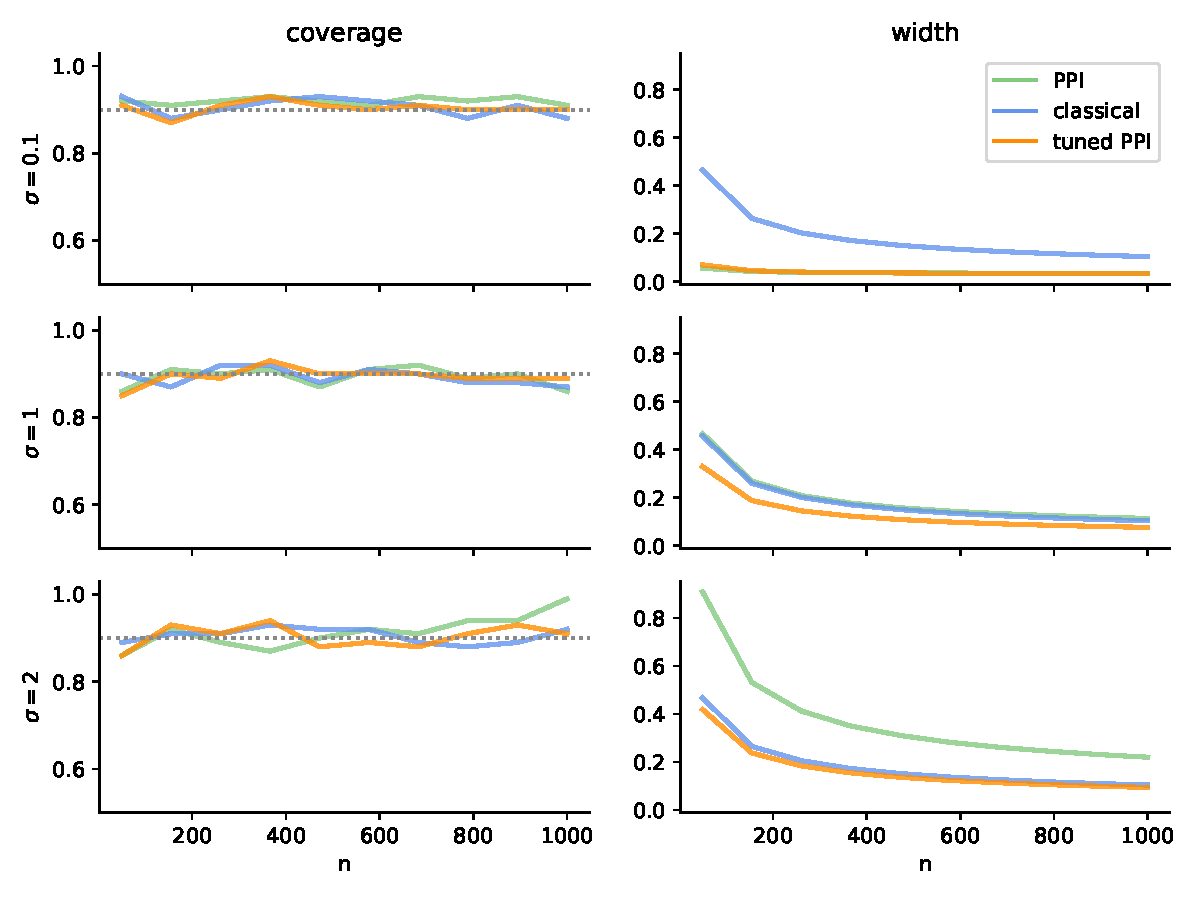
\includegraphics[width=0.9\textwidth]{plots/tuned-PPI-mean.pdf}
    \caption{Mean estimation simulation study.  The left column shows
      coverage, the right column shows confidence interval width.  The top,
      middle, and bottom rows correspond to noise levels $\sigma=0.1$,
      $\sigma=1$, and $\sigma=2$, respectively.}
    \label{fig:mean_estimation}
\end{figure}

\paragraph{Linear regression.}

The goal is to estimate the coefficients of a linear regression model $Y =
X^\top \theta + \epsilon$, where $X \sim \normal(0,I_d)$, $\theta \in \R^d$,
and $\epsilon \sim \normal(0,1)$, in dimension $d = 2$.
%
We use predictions $f(X_i) = X_i^\top \theta + \epsilon_i$,
where $\epsilon_i \sim \normal(-2, \sigma^2)$.
%
We vary the noise level $\sigma \in \{0.1, 0.5, 1\}$, plotting
results in Figure~\ref{fig:linear_regression}.
%
The results are qualitatively similar to those in
Figure~\ref{fig:mean_estimation}: \ppipp adaptively interpolates between
classical inference and standard PPI as the noise level changes,
outperforming both.

\begin{figure}[t]
  \centering
  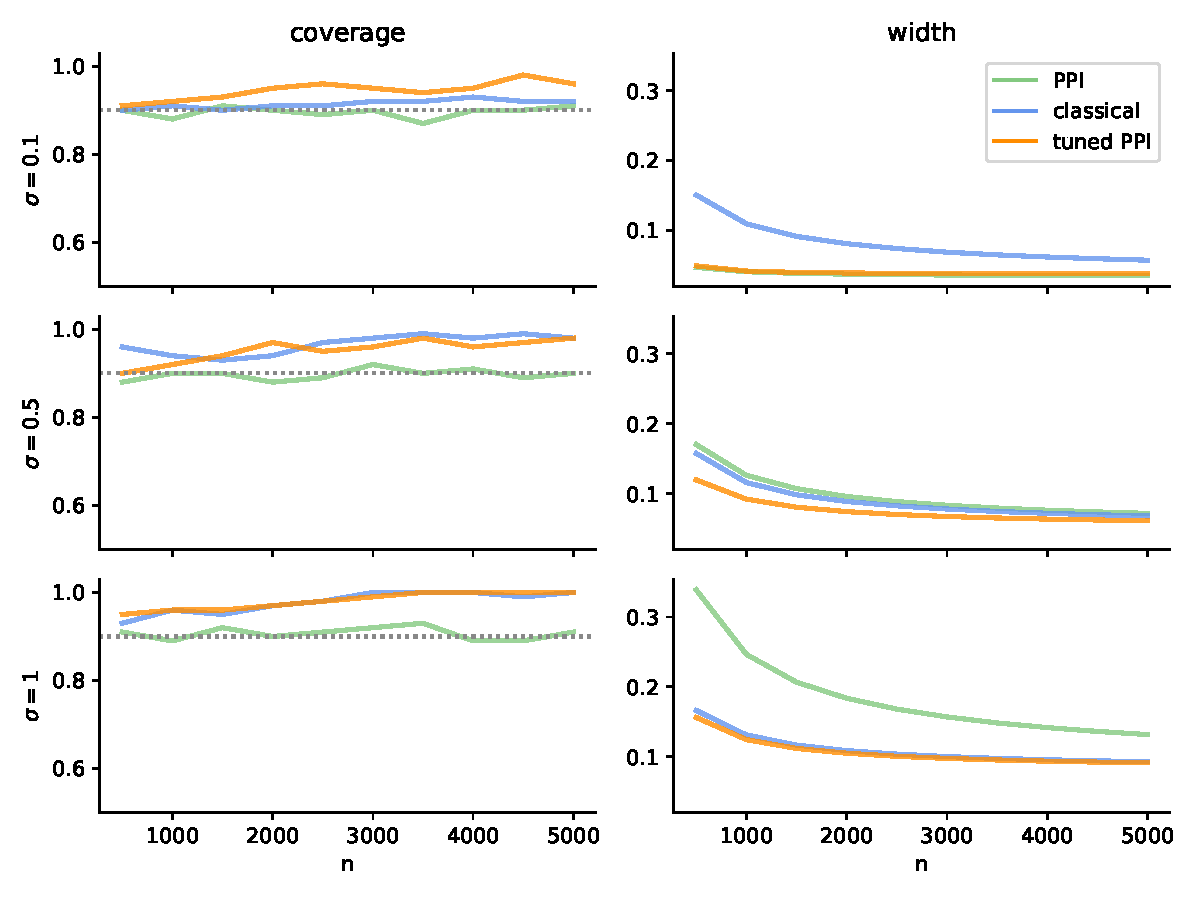
\includegraphics[width=0.9\textwidth]{plots/tuned-PPI-ols.pdf}
  \caption{Linear regression simulation study.  The left column shows
    coverage, the right column shows confidence interval width. The top,
    middle, and bottom rows correspond to noise levels $\sigma=0.1$,
    $\sigma=0.5$, and $\sigma=1$, respectively.}
  \label{fig:linear_regression}
\end{figure}

\paragraph{Logistic regression.}

The goal is to estimate the coefficients of a logistic regression model,
$\P(Y=1) = \mu_\theta(X)$, where $\mu_\theta(x) = \frac{e^{\theta^\top x}}{1
  + e^{\theta^\top x}}$ for $\theta \in \R^d$ with dimension $d = 2$.
%
We draw $X \sim \normal(0,I_d)$ and to simulate a binary classifier $f$ with
error $\sigma$, we set the predictions $f(X_i)$ to be $Y_i$ but randomly
flipped with probability $\sigma$.
%
We vary the flipping probability $\sigma \in \{0.01, 0.1, 0.2\}$, presenting
results in Figure~\ref{fig:logistic_regression}.
%
As before, \ppipp successfully adapts to the varying noise in the
predictions.

\begin{figure}[t]
    \centering
    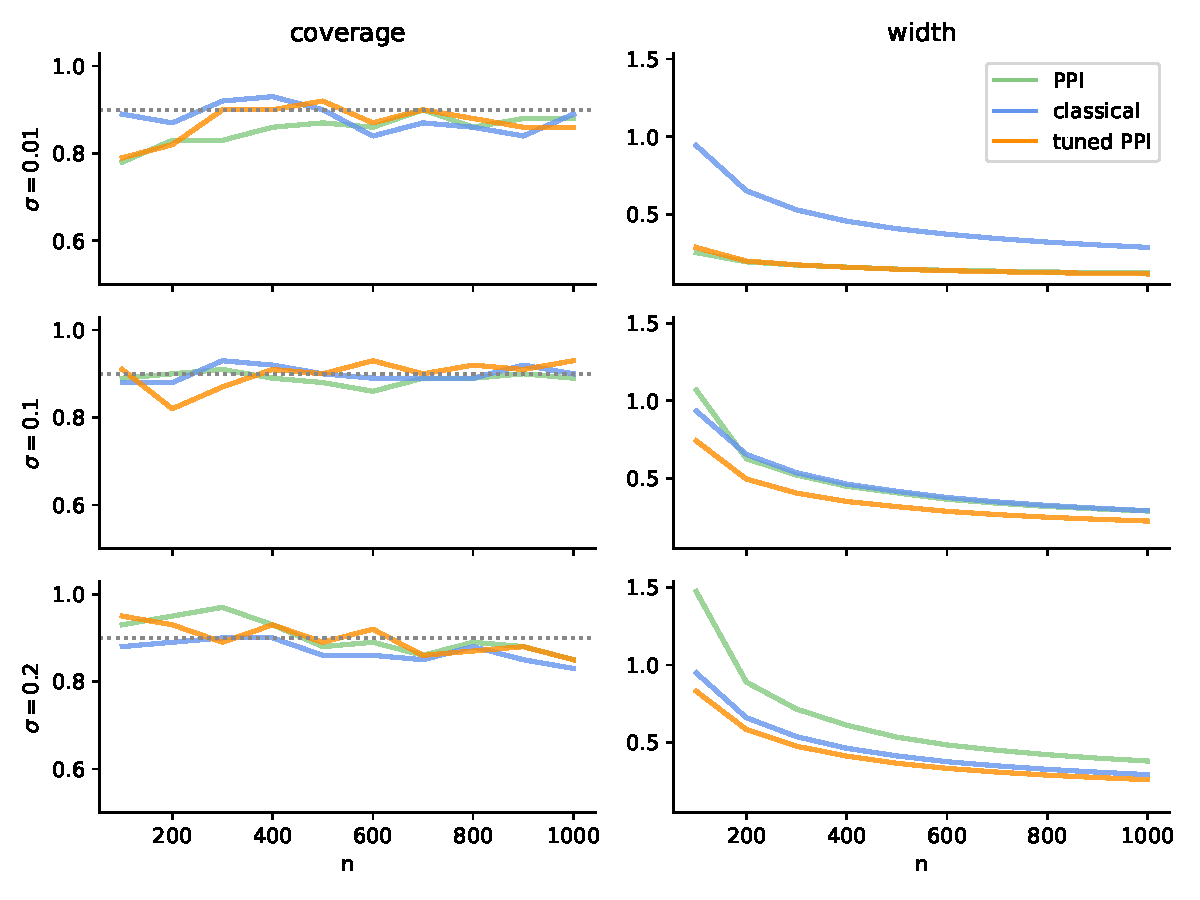
\includegraphics[width=0.9\textwidth]{plots/tuned-PPI-logistic.pdf}
    \caption{Logistic regression simulation study. The left column shows
      coverage, the right column shows confidence interval width. The top,
      middle, and bottom rows correspond to noise levels $\sigma=0.01$,
      $\sigma=0.1$, and $\sigma=0.2$, respectively.}
    \label{fig:logistic_regression}
\end{figure}

\subsubsection{Real data experiments}

We now revisit five experiments on real data that
\citeauthor{AngelopoulosBaFaJoZr23} perform~\citep{AngelopoulosBaFaJoZr23},
where we replicate their experimental settings, comparing to
classical inferential approaches (that do not use the unlabeled data)
as well.

\paragraph{Mean estimation on deforestation data.}

The goal is to estimate the mean deforestation rate in the Amazon based on
satellite imagery data~\cite{AngelopoulosBaFaJoZr23}.  The dataset includes
$1596$ total pairs of observations and predictions, where the observations
indicate whether deforestation occurred in a given randomly sampled region
and the predictions are probits corresponding to these indicators.  We take
these predictions from the same gradient-boosted classifier as
in~\cite{AngelopoulosBaFaJoZr23}, which is fit on a publicly available
machine learning system that released tree canopy forest cover predictions
at 30m resolution in the years 2000 and 2015.  Generally, when the amount of
forest cover in 2015 is substantially lower than in 2000, the model predicts
that deforestation occurred.

Of the $1596$ total data points, we vary $n$, and then
randomly take a labeled subset of size $n$ and
use $N=1596-n$ as unlabeled.
%
Figure~\ref{fig:mean_estimation_real_data} shows the results of the
procedures over $100$ random splits into labeled and unlabeled data. For small
$n$, \ppipp behaves similarly to standard PPI. When $n$ is large, meaning
the unlabeled dataset size $N$ is small, classical inference outperforms
standard PPI; \ppipp outperforms both.

\begin{figure}[H]
    \centering
    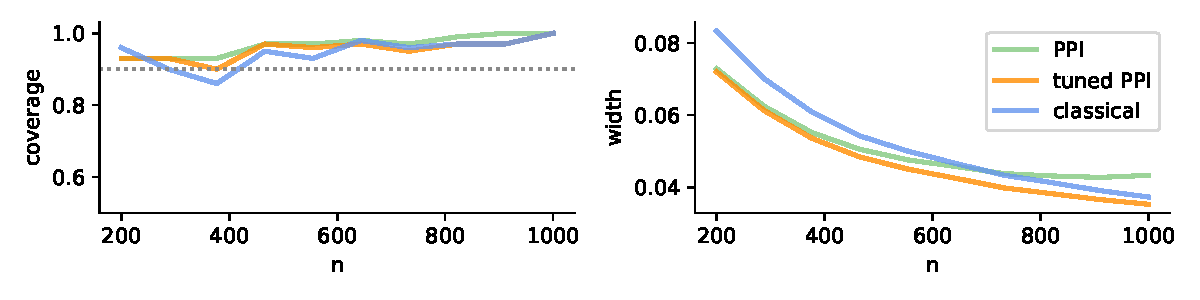
\includegraphics[width=0.9\textwidth]{plots/tuned-PPI-forest.pdf}
    \caption{Mean estimation on deforestation data. The left panel shows coverage and the right shows width.}
    \label{fig:mean_estimation_real_data}
\end{figure}

\paragraph{Mean estimation on galaxy data.}

The goal is to estimate the fraction of spiral galaxies in the local universe based on images from the Sloan Digital Sky Survey (SDSS) and a pre-trained ResNet classifier, as in~\cite{AngelopoulosBaFaJoZr23}.
%
The scale of the universe makes human labeling of galaxies impossible, so
scientists wish to use a computer-vision-based classifier to study the
development of the universe. The classifier ingests images of galaxies and
outputs an estimated probability that the galaxy is spiral.
%
The dataset includes 1,364,122 total observations, of which we randomly take $n$ to serve as the labeled data and $N=1,\!364,\!122-n$ as the unlabeled data, for varying $n$.
We show the results in Figure~\ref{fig:mean_estimation_real_data_galaxies} over $100$ random splits into labeled and unlabeled data.
%
As the predictions are very accurate in this problem, \ppipp and standard PPI are basically indistinguishable, and both are significantly more powerful than classical inference.

\begin{figure}[H]
    \centering
    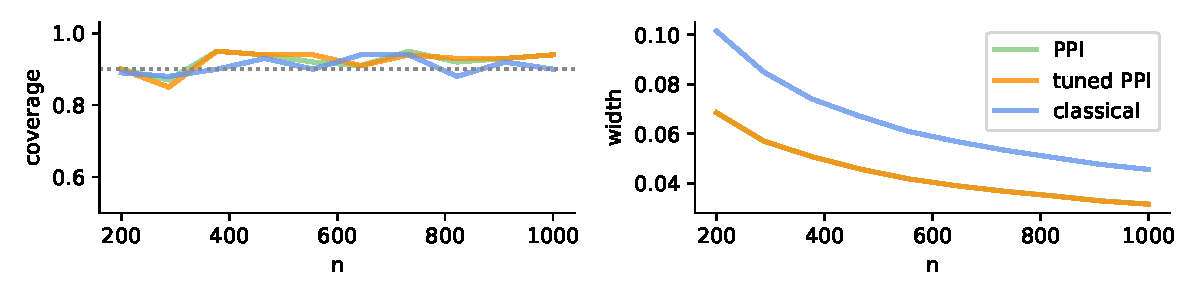
\includegraphics[width=0.9\textwidth]{plots/tuned-PPI-galaxies.pdf}
    \caption{Mean estimation on galaxy data. The left panel shows coverage and the right shows width.}
    \label{fig:mean_estimation_real_data_galaxies}
\end{figure}

\paragraph{Odds ratio estimation on AlphaFold data.}

The goal is to estimate the odds ratio of a protein being phosphorylated and
being part of an intrinsically disordered region (IDR) using the predictions
from AlphaFold~\cite{JumperEvEtAl21}, as in~\cite{AngelopoulosBaFaJoZr23}.
The cost of measuring protein structure has prompted scientists to
increasingly rely on AlphaFold's predictions to study the
natural distribution of protein structures. The data set includes $10802$
total observations of ground-truth IDR indicators and corresponding
AlphaFold predictions, which we randomly split into $n$ labeled
and $N=10802-n$ unlabeled data points, for varying $n$.  See
Figure~\ref{fig:odds_ratio_estimation_real_data} for the results over $100$
random splits into labeled and unlabeled data. For moderately low values of
$n$, tuned PPI and standard PPI have similar performance, both outperforming
classical inference. As $n$ becomes large, tuned PPI gradually becomes more
powerful than both alternatives.

The original PPI confidence sets~\citep{AngelopoulosBaFaJoZr23} are formed by splitting the error budget between two means and post-processing them to recover a confidence set for the odds ratio. 
We do not use this overly conservative approach; instead, we derive an asymptotically exact confidence set for the odds ratio using the delta method.
See Appendix~\ref{app:odds-ratio} for details.

\begin{figure}[H]
    \centering
    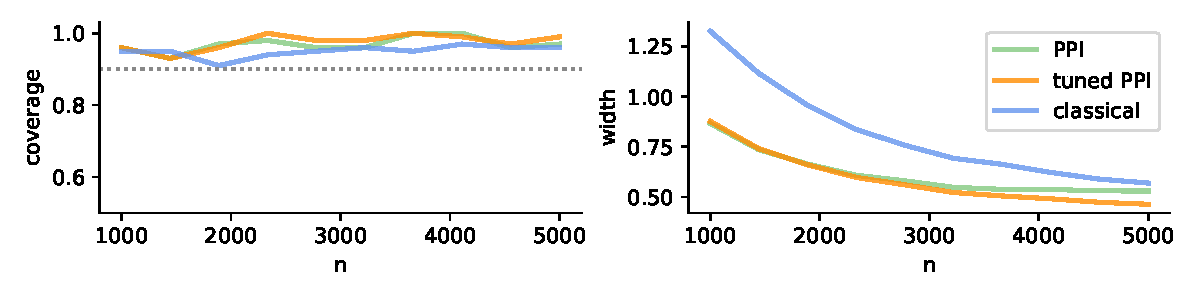
\includegraphics[width=0.9\textwidth]{plots/tuned-PPI-alphafold.pdf}
    \caption{Odds ratio estimation on AlphaFold data. The left panel shows coverage and the right shows width.}
    \label{fig:odds_ratio_estimation_real_data}
\end{figure}


\paragraph{Linear regression on census data.}

In this experiment, the goal is to estimate the coefficients of a linear
regression model relating age (1-99) and sex (M/F) to income based on census
data from California, as in~\cite{AngelopoulosBaFaJoZr23}. We download the
data through the Folktables~\cite{DingHaMiSc21} interface and use an XGBoost
model~\cite{ChenGu16} taking as input the ten covariates available in
Folktables (including age, sex, the binary indicator of private health
insurance) to produce predictions.  We train the model on the entire census
dataset in the year 2018 and use it to predict income for the year
2019.  The 2019 data includes $377,\!575$ observations, of which we randomly
take $n$ as labeled and $N=377,\!575-n$ as unlabeled, for varying $n$.  We show
the results in Figure~\ref{fig:ols_real_data} over $100$ random splits into
labeled and unlabeled data. \ppipp is visually indistinguishable from
standard PPI with $\lambda=1$.

\begin{figure}[ht]
    \centering
    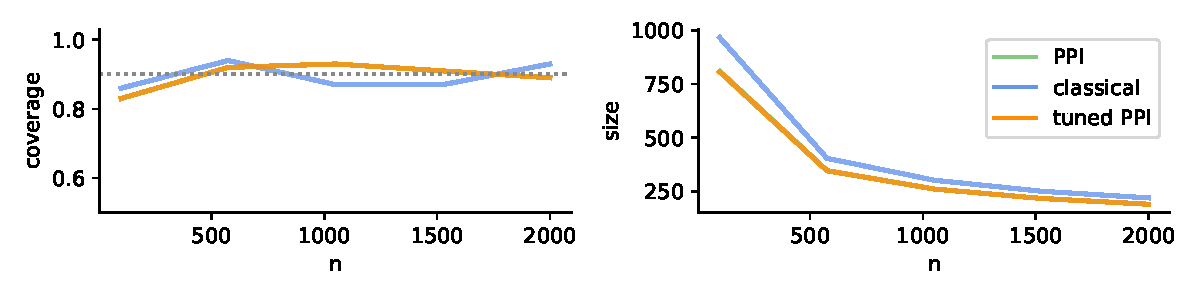
\includegraphics[width=0.9\textwidth]{plots/census_income_tuned.pdf}
    \caption{Linear regression on census data. The left panel shows coverage and the right shows width.}
    \label{fig:ols_real_data}
\end{figure}

\paragraph{Logistic regression on census data.}
The goal is to estimate the coefficients of a logistic regression model relating income (\$) to the binary indicator of private health insurance based on census data.
The setup otherwise resembles the previous experiment: we train an XGBoost model to predict income from ten other covariates, we have $377,\!575$ total observations, and so on.
Figure~\ref{fig:logistic_real_data} shows the results over $100$ random splits into labeled and unlabeled data. Tuned PPI behaves similarly to PPI, and both are more powerful than classical inference for all values of $n$.

\begin{figure}[ht]
    \centering
    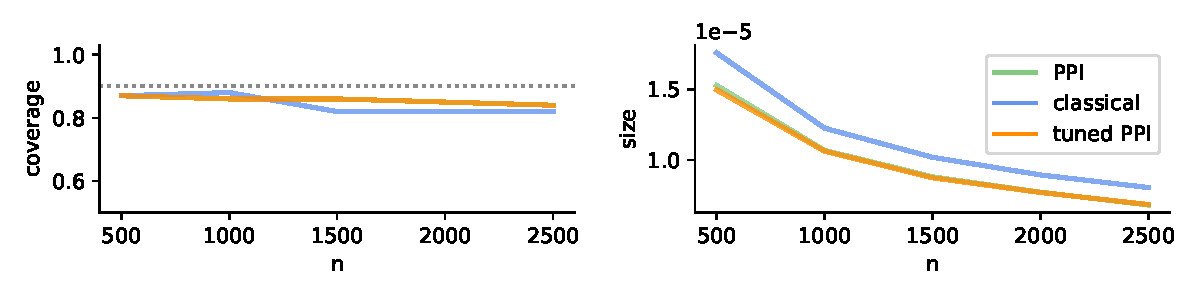
\includegraphics[width=0.9\textwidth]{plots/census_healthcare_tuned.pdf}
    \caption{Logistic regression on census data. The left panel shows coverage and the right shows width.}
    \label{fig:logistic_real_data}
\end{figure}

\subsection{Comparison to confidence sets from testing}

The final comparison is to the naive implementation of prediction-powered
inference~\citep[Algorithm 3]{AngelopoulosBaFaJoZr23}.  We do not apply
power tuning in this comparison as the goal is to understand the independent
effect of the gridding procedure, which tests for ``each'' $\theta$ whether
$\nabla \LPP(\theta) = 0$ is plausible, versus the technique proposed
herein. The gridding means the original PPI method has much larger
computational cost than the proposed method, while it is also less accurate
(leading to larger sets, as in Figure~\ref{fig:comparison}).  This follows
because, to remain valid, the gridding method necessarily includes
an extra grid point along each dimension.  Furthermore, the method often
outputs infinite sets because, in an effort to avoid an infinite runtime,
the algorithm simply terminates grid refinement after a certain number of
iterations.  See Figure~\ref{fig:comparison} for the median interval width
for varying dimension $d$ and limit on the number of grid points before the
algorithm returns an infinite set.

\begin{figure}[ht]
    \centering
    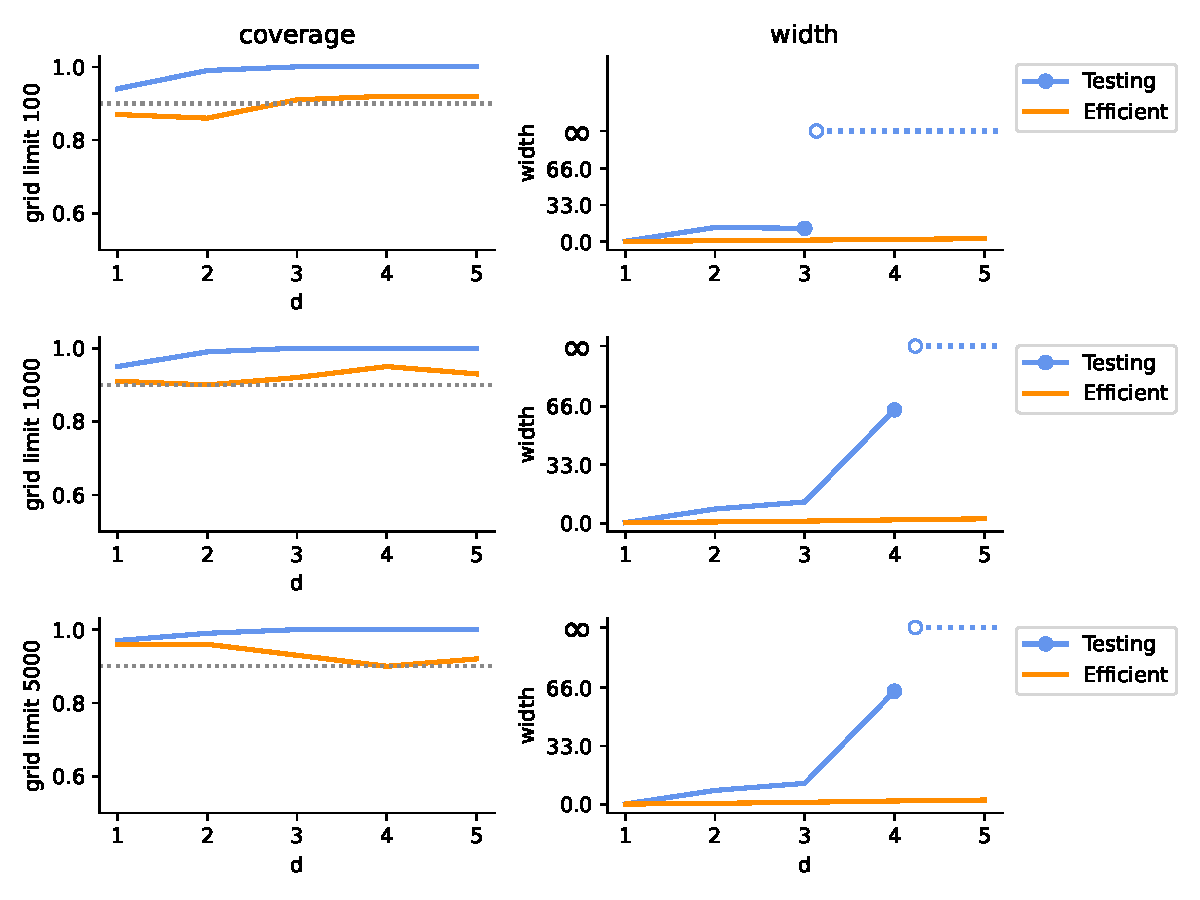
\includegraphics[width=0.9\textwidth]{plots/eff-comparison.pdf}
    \caption{Comparison of \ppipp logistic regression, as in
      Algorithm~\ref{alg:glms}, and standard PPI logistic
      regression~\cite[Algorithm 3]{AngelopoulosBaFaJoZr23}. The left panel
      shows coverage and the right shows width.}
    \label{fig:comparison}
\end{figure}

\section*{Acknowledgements}
The authors would like to acknowledge the support of the Mohamed bin Zayed
University of Artificial Intelligence and president Eric Xing as well as
Barbara Engelhardt for their organization of the Michael Jordan Symposium,
which led to this idea and collaboration.  We also thank Michael Jordan for
his encouragement.  JCD's work was additionally supported by the Office of
Naval Research Grant N00014-22-1-2669 and as a Thomas and Polly Bredt
Faculty Scholar.
% We would also like to thank Mike Jordan for lubricating our discussions with ``liquid happiness.''
